\section{草稿}
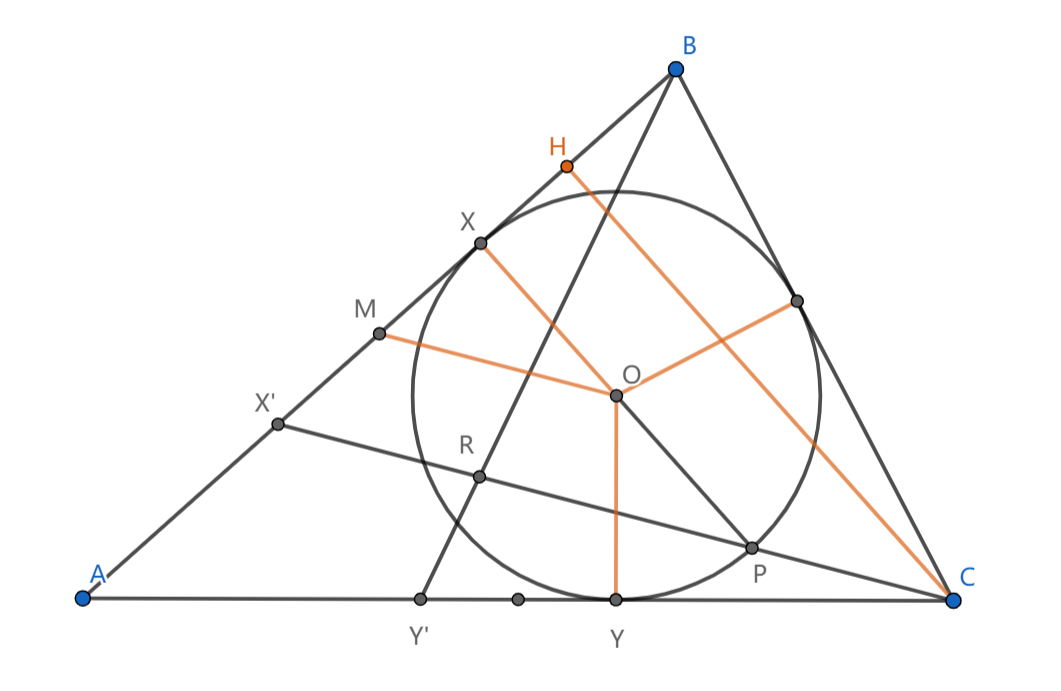
\includegraphics[width=0.8\textwidth]{pictures/6-30.1.png}

\begin{proof}
    不失一般性地,认为内切圆的半径为 $1$,认为三条垂线两两夹角为 $2\theta_1, 2\theta_2, 2\theta_3$,并将 $\tan \theta_1$ 简记为 $t_1$,$t_2, t_3$ 以此类推.

    于是可以得到以下角度或长度的值或关系:
    \[\angle A = \pi - 2\theta_1, \quad \angle ABC = \pi - 2\theta_2, \quad \angle ACB = \pi - 2\theta_3\]
    \[AX = AY = t_1, \quad BX = AX' = t_2, \quad CY = AY' = t_3\]
    \[\theta_1 + \theta_2 + \theta_3 = \pi\]

    接下来先尝试证明 $XO$ 与 $OP$ 共线.

    考虑过 $C$ 作直线 $AB$ 的垂线,令垂足为 $H$,考虑直角三角形 $\Delta CHX'$ 中 $\angle HX'C$ 的余切值.
    \[CH = AC \times \sin \angle A = (t_1 + t_3) \cdot \sin(\pi - 2\theta_1) = (t_1 + t_3) \sin 2\theta_1\]
    \[X'H = AH - AX' = AC \times \cos \angle A - AX' = (t_1 + t_3) \cdot \cos(\pi - 2\theta_1) - t_2 = -(t_1 + t_3) \cos 2\theta_1 - t_2\]

    所以
    \[\cot \angle HX'C = \frac{X'H}{CH} = -\cot 2\theta_1 - \frac{t_2}{(t_1 + t_3)\sin 2\theta_1}\]

    然后借助
    \[\cot 2\theta_1 = \frac{1 - t_1^2}{2t_1}, \quad \sin 2\theta_1 = \frac{2t_1}{1 + t_1^2}, \quad t_3 = \tan(\pi - \theta_1 - \theta_2) = \frac{t_1 + t_2}{t_1t_2 - 1}\]

    化简得
    \[\cot \angle HX'C = \frac{t_1 - t_2}{2}\]

    再考虑直角三角形 $\Delta MXO$ 中 $\angle OMX$ 的余切值.
    \[OX = 1\]
    \[MX = \frac{XX'}{2} = \frac{AX - AX'}{2} = \frac{t_1 - t_2}{2}\]

    所以
    \[\angle BX'C = \angle XMO \Rightarrow MO \parallel X'C\]

    稍做分析可得 $OP$ 与 $XO$ 共线.

    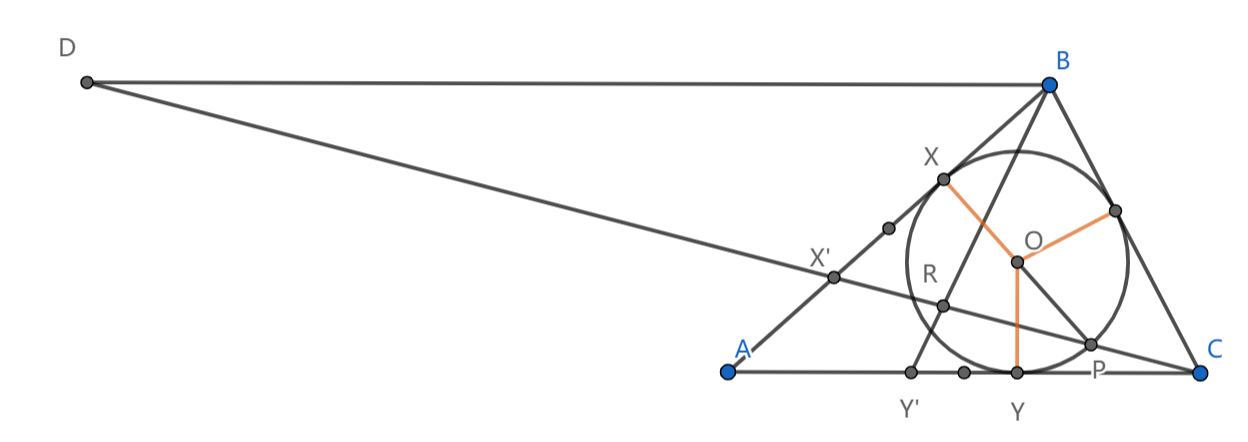
\includegraphics[width=0.9\textwidth]{pictures/6-30.2.png}

    现在延长线段 $CX'$ 与过 $B$ 关于 $AC$ 的平行线交于点 $D$.

    运用平面几何知识可得
    \[DR = \frac{t_1 + t_3}{t_1 + t_2 + t_3} CD\]
    \[DX' = \frac{t_1}{t_1 + t_2} CD\]
    \[CD = \frac{t_1 + t_2}{t_2} CX'\]

    所以
    \[X'R = DR - DX' = \frac{t_3}{t_1 + t_2 + t_3} CX' = \frac{t_1 + t_2}{t_1t_2} CX'\]

    同样的,
    \[CP = CX' \cdot \frac{CH - 2}{CH} = \left(1 - \frac{1 + t_1^2}{t_1(t_1 + t_3)}\right) CX' = \frac{t_1 + t_2}{t_1t_2} CX'\]

    从而得到
    \[X'R = CP\]
\end{proof}

\textbf{格点问题}
\begin{proof}[解]
    注意到:将所有格点进行行、列对换之后长方形不被破坏,因此如果一种涂色方法符合题意,那么对它进行行、列对换之后也依旧符合题意.

    假设一种涂色方案满足题意,能够通过有限次行、列对换将它变形成如下形式:

    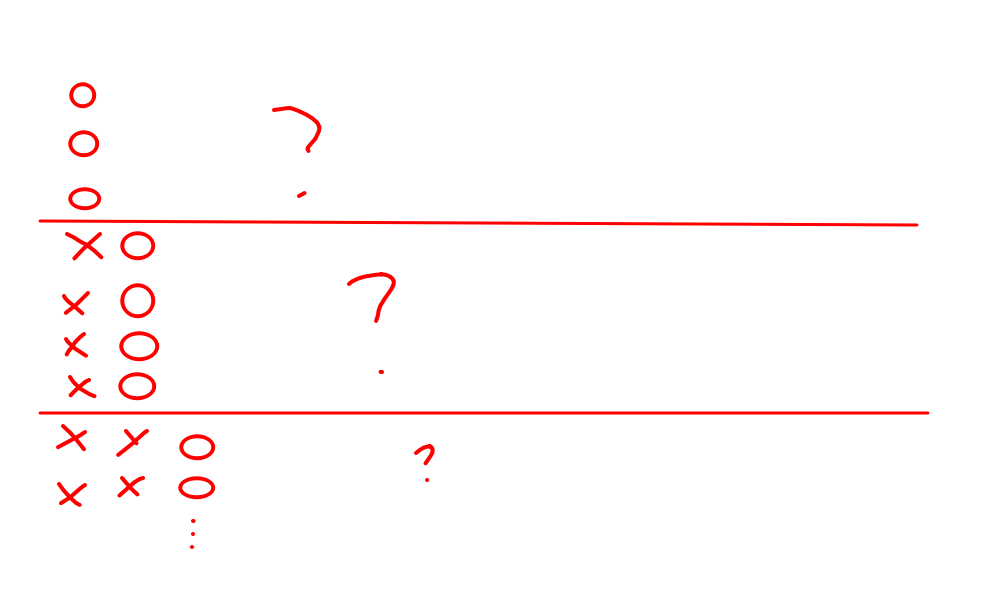
\includegraphics[width=0.8\textwidth]{pictures/6-30.3.png}

    圆圈代表红点,叉号代表非红点.

    我们用上图的方式对格点区域从上往下进行排序,第 $k$ 个区域的前 $k-1$ 列全空,第 $k$ 列全红,总共有 $n$ 个区域,其中 $n \leqslant 40$.

    为了方便计算,认为行数为 $2040$,列数为 $40$.

    现在考虑第 $k$ 个区域从第 $k+1$ 列往右的部分. 因为第 $k$ 列的格点全被涂上了红色,因此右侧不可能出现两个红色格点在同一列的现象,所以右侧红色格点个数的最大值就是剩余列数,即 $40-k$.

    现在我们用 $x_k$ 来指代第 $k$ 个区域所占用的行数.

    可以发现,第 $k$ 个区域红色格点数目的最大值为 $x_k + 40 - k$.

    所以总共格点数小于等于
    \[\sum_{k=1}^{n} \bigl(x_k + 40 - k\bigr) = \sum_{k=1}^{n} x_k + \frac{79n-n^2}{2}\]

    通过简单分析可得,$x_k$ 的求和的最大值为 $2040$.

    又因为 $(80n-n^2)/2$ 随着 $n$ 取值的增大而增大,因此取最大值 $n = 40$ 得到 $780$.

    因此红色格点数的最大值不超过 $2040 + 780 = 2820$.

    然后只要构造出一种染色方案使得总共 $2820$ 个格点被染上红色且满足题意即可,这里给出一种方案.
    \[x_1, x_2, \cdots, x_{39} = 40, \quad x_{40} = 480\]
    
    对第 $k$ 个区域第 $k$ 列以右的部分从左下往右上染色,类似于函数 $y = x$.
\end{proof}